\documentclass[12pt,a4paper]{article}
\usepackage[utf8]{inputenc}
\usepackage[german]{babel}
\usepackage{amsmath}
\usepackage{amsfonts}
\usepackage{amssymb}
\usepackage{graphicx}
\usepackage{epstopdf}
\usepackage{enumitem}
\usepackage{gensymb}
\usepackage{float}
\usepackage{tikz}
\usetikzlibrary{arrows,shapes,positioning,shadows,trees}

\tikzset{
  basic/.style  = {draw, text width=2cm, drop shadow, font=\sffamily, rectangle},
  root/.style   = {basic, rounded corners=2pt, thin, align=center, fill=blue!30},
  level 2/.style = {basic, rounded corners=6pt, thin,align=center, fill=cyan!60, text width=5em},
  level 3/.style = {basic, thin, align=left, fill=gray!20, text width=4.5em},
  level 3w/.style = {basic, thin, align=left, fill=red!40, text width=4.5em}
}

\author{Philipp Oldenburg, Patrick Zumsteg, Simon Wallny}
\title{Gruppe „Denial of Service“}
\date{Frühjahrssemester 2015}
\begin{document}
\maketitle
\tableofcontents
\section{Vorwort}
Das Projekt „Denial of Service“, entstand im Rahmen der Vorlesung „Internet-Technologien“ an der Universität Basel im Frühjahrssemester 2015.\hfill\\
Die bearbeitende Gruppe besteht aus Philipp Oldenburg, Patrick Zumsteg und Simon Wallny.
\newpage
\section{Definition}
,,Denial of Service`` (engl. \textit{Verweigerung des Dienstes}) beschreibt eine Art eines Angriffs auf einen öffentlich verfügbaren Dienst im Internet. Ziel dieses Angriffes ist es, dass der Dienst des Ziels, etwa ein Online-Shop, zeitweise nicht mehr zur Verfügung steht.  Dies wird auf unterschiedliche Weise bewerkstelligt, aber die zugrundeliegende Idee ist in jeden Fall dieselbe: Die Ressourcen des Dienstes, Prozessorauslastung, Speicher oder Bandbreite, die immerhin über das Internet zur Verfügung gestellt werden, werden in unverhältnismäßigem Maße beansprucht, sodass tatsächlichen Nutzern des Dienstes keine Kapazitäten mehr zur Verfügung stehen.\\
Erfolgt ein solcher Angriff über mehrere Rechner an verschiedenen Orten, spricht man von einer ,,Distributed Denial of Service``-Attacke (engl. \textit{Verteilte Verweigerung des Dienstes}), kurz DDoS.\\
Das Ausführen von Angriffen dieser Art in öffentlichen Netzen sind in der Schweiz gemäß Artikel 144 des Strafgesetzbuches strafbar.
\section{Angriffs- und Verteidigungs-Strategien anhand einiger Beispiele}
DoS-Angriffe können über verschiedene Wege gefahren werden, und auf unterschiedlichen Ebenen unterschiedliche Ressourcen blockieren. Im folgenden sind einige Beispiele aufgeführt.
\subsection{Applikationsebene - Slow Headers}
\subsubsection*{Angriff}
Ein ,,Slow Headers``-Angriff ist ein auf Webserver spezialisierter, besonders eleganter Angriff, der dem Angreifer kaum Ressourcen abverlangt. Hierbei wird dem Ziel ein Strom von unfertigen Headern von HTTP-Get Anfragen geschickt. Der Server muss, damit der Angriff effektiv ist, konfiguriert sein die Verbindung offen zu halten und auf den Rest der Anfrage zu warten. Diese Verbindungen lassen sich nun offen halten, indem bevor der timeout erfolgt, der mehrere Minuten lang sein kann, ein weiterer Teil der Anfrage geschickt wir, wobei der Header allerdings immer noch nicht geschlossen wird. Der Webserver, der nur eine endliche Menge Verbindungen halten kann, wird so für normale Nutzer unzugänglich.
\subsubsection*{Verteidigung}
TODO
\subsection{Transportebene - Syn Flood.}
\subsubsection*{Angriff}
Syn Flood (engl. \textit{Syn Flut}) ist ein simpler Angriff, bei dem von dem normalen TCP-Handshake der erste Schritt von Seitens des Angreifers so schnell wie möglich wiederholt wird. Das Ziel ertrinkt nun in der Flut von Verbindungsanfragen und kann nicht mehr auf alle antworten, auch nicht auf die vereinzelten echten Anfragen seiner Nutzer.
\subsubsection*{Verteidigung}
Momentan sind mehrere Wege bekannt, sich gegen eine SYN-Flut zu wehren. Ein naiver Ansatz wäre natürlich, die älteste der halboffenen Verbindungen (die also noch kein ACK vom Client erhalten haben) einfach zu recyclen und für ein neu ankommendes SYN zu verwenden. Hierbei hat natürlich der Client, dem die Verbindung ursprünglich gehörte, das Nachsehen, und im Falle einer heftigen SYN-Flut ist das Backlog des Servers immer noch (fast) nur mit ,,böswilligen`` Verbindungen befüllt.\\
Gegen SYN-Floods gibt es aber schon seit langer Zeit eine "Wunderwaffe", bekannt als SYN-Cookies. Die Idee hierbei ist, dass der Server die Sequenznummer seines SYN-ACK-Pakets anhand eines üblicherweise im Minutentakt inkrementierten Zeitstempels, seiner eigenen und der Adresse des Clients berechnet. Ein Client, der wirklich eine Verbindung will, kann würde die Sequenznummer dieses Pakets um eins erhöhen und als ACK-Nummer in seinem ACK-Paket zurückschicken. Der Server kennt nun ja sowohl den aktuellen(oder letzten) Zeitstempel, als auch Quell-und Zieladressen, kann also nachrechnen, ob er diesem Client vor kurzem ein SYN-ACK geschickt haben kann.
\subsection{Netzwerkebene - ICMP Flood}
\subsubsection*{Angriff}
ICMP Flood (engl. \textit{ICMP Flut}) Bei einem ICMP Smurf-Angriff kann ein schlecht konfiguriertes Netzwerk ausgenutzt werden, um ein Ping-Packet das so aussieht, als komme es vom Ziel, an alle Rechner des Netzes zu schicken, die allesamt antworten und das Ziel damit stark belasten.
\subsubsection*{Verteidigung}
Obwohl Slow-Header-Angriffe extrem mächtig sind und einen Server mühelos in die Knie zwingt, solange die Angreiferseite mehr Ports offen halten kann als der verteidigende Anbieter, ist es leider (oder zum Glück) sehr leicht, sich gegen diese Attacken zu immunisieren. Da ein Slow-Headers-Angriff alle Verbindungen besetzt und offen hält, die der Server bereitstellt, muss dieser nichts weiter tun, als die Anzahl an simultanen Verbindungen, die ein Client (sprich: eine IP-Adresse, was nicht unproblematisch ist) offen halten kann, zu begrenzen. Hierfür gibt es beispielsweise das Apache-Modul \textit{mod\_qos}.\\
Allerdings ist diese Verteidigung nicht narrensicher; einerseits kann es sein, dass ein Serviceanbieter damit rechnet, mit vielen Clients gleichzeitig zu arbeiten, die sich hinter einem NAT befinden, also aus Sicht des Servers von der gleichen IP aus kommunizieren. In diesem Fall müsste er eine große Anzahl an simultanen Verbindungen zulassen, was seine Verteidigung natürlich stark schwächt. Außerdem ist man gegen einen verteilten Angriff immer noch nur mittelmäßig geschützt: Sei $x$ die Anzahl Verbindungen, die pro IP simultan geöffnet sein dürfen, und $M$ die Anzahl Verbindungen, zu der der Server insgesamt fähig ist. Dann braucht es höchstens $\frac{M}{x}$ Angreifer-IPs, um den Host lahmzulegen. Die maximale Anzahl an Verbindungen, die der Server eingehen kann, ist zwar frei wählbar, allerdings müssen hinter dieser Zahl natürlich entsprechenden Systemressourcen stehen, und das Problem wird nur auf CPU/RAM verschoben.
\section{Bekannte Anwendungen}
\subsection{Low Orbit Ion Cannon}
Die LOIC ist ursprünglich eine open-source Software für Belastungstests. Unsere Tests haben wir allerdings mit einer abgewandelten Version der Anwendung durchgeführt, einem von einer sich zum freien Internetkollektiv Anonymous bekennender Gruppe Hacktivisten entwickeltes DoS-Angriffstool. Anders als bei den meisten frei verfügbaren Tools war ihre Bestimmung niemals Belastungstests, sondern das anrichten von Schaden an politisch motivierten Zielen. Während diese Ion Cannon in erster Linie für verteilte Angriffe, DDoS, gedacht ist, und sich zwecks dessen in einen ,,Hive Mode`` schalten lässt, bei dem ein Angriff zentral synchronisiert von vielen Teilnehmern gleichzeitig gestartet wird, lassen sich auch mit einer einzigen Anwendung messbare Ergebnisse erzielen.\\
Wir haben den uns zur Verfügung gestellten Rechner über eine lokale Verbindung mit der LOIC angegriffen, und folgende Messwerte erhalten.\\
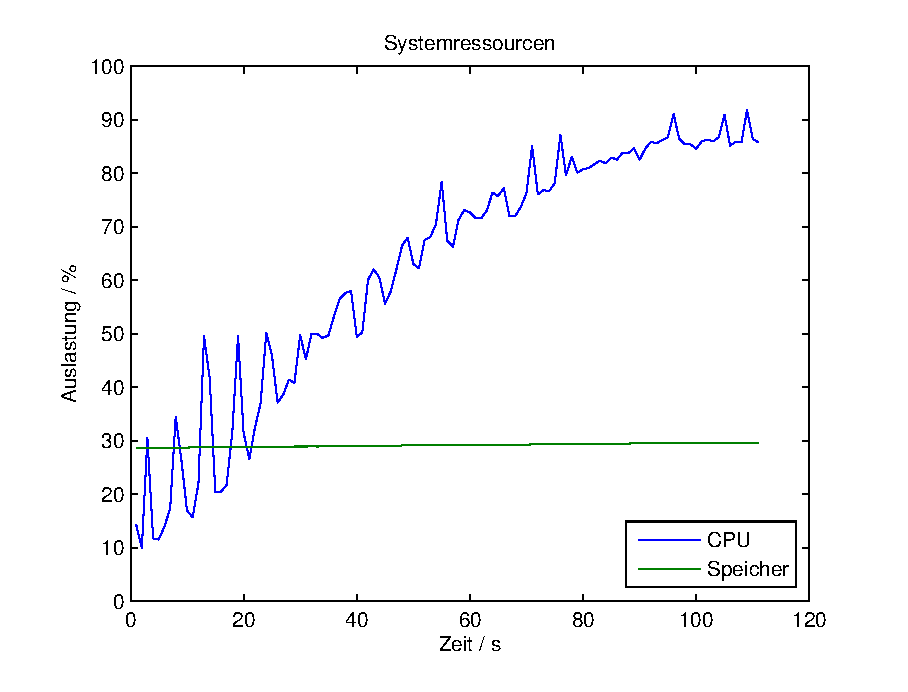
\includegraphics[scale=0.9]{MatLab/LOICVictimSys.eps}\\
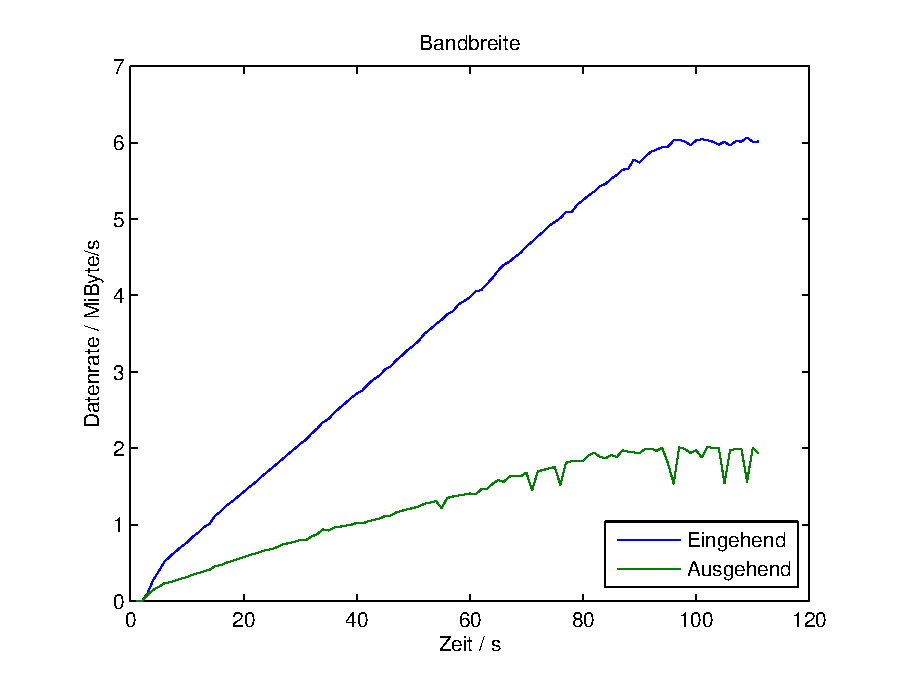
\includegraphics[scale=0.9]{MatLab/LOICVictimBand.eps}\\
Dieser vereinzelte Angriff war nicht genug, damit der Server den Dienst vollständig quittiert, allerdings hat er schon bei diesen harmlosen Dimensionen merklich langsamer geantwortet als sonst.
\subsection{Open Web Application Security Project}
SwitchBlade, lizenziert von ProactiveRISK, ist eine Anwendung in Rahmen des OWASP um Belastungstests für eigene Webserver auszuführen. Dazu führt es einen ,,Slow Headers``-Angriff aus, und legte in unseren Tests einen frisch aufgesetzten, ungeschützten Apache-Server binnen Sekunden gründlich lahm. Die Threadkonfiguration des frisch gestarteten Servers bestand aus zwei Kindprozessen mit jeweils 25 Threads, hier auf 10 gekürzt.
\begin{figure}[H]
\centering
\begin{tikzpicture}[
  level 1/.style={sibling distance=24mm},
  edge from parent/.style={->,draw},
  >=latex]

% root of the the initial tree, level 1
\node[root] {Main Thread}
% The first level, as children of the initial tree
  child {node[level 2] (c1) {Child 1}}
  child {node[level 2] (c2) {Child 2}};

% The second level, relatively positioned nodes
\begin{scope}[every node/.style={level 3}]
\node [below of = c1, yshift=10pt] (c11) {Idle};
\node [below of = c11, yshift=15pt] (c12) {Idle};
\node [below of = c12, yshift=15pt, fill=green!20] (c13) {Reply};
\node [below of = c13, yshift=15pt] (c14) {Idle};
\node [below of = c14, yshift=15pt] (c15) {Idle};
\node [below of = c15, yshift=15pt] (c16) {Idle};
\node [below of = c16, yshift=15pt] (c17) {Idle};
\node [below of = c17, yshift=15pt] (c18) {Idle};
\node [below of = c18, yshift=15pt] (c19) {Idle};
\node [below of = c19, yshift=15pt] (c110) {Idle};

\node [below of = c2, yshift=10pt] (c21) {Idle};
\node [below of = c21, yshift=15pt] (c22) {Idle};
\node [below of = c22, yshift=15pt] (c23) {Idle};
\node [below of = c23, yshift=15pt] (c24) {Idle};
\node [below of = c24, yshift=15pt] (c25) {Idle};
\node [below of = c25, yshift=15pt] (c26) {Idle};
\node [below of = c26, yshift=15pt] (c27) {Idle};
\node [below of = c27, yshift=15pt] (c28) {Idle};
\node [below of = c28, yshift=15pt] (c29) {Idle};
\node [below of = c29, yshift=15pt] (c210) {Idle};

\end{scope}
\end{tikzpicture}
\end{figure}
\noindent Nachdem der Angriff gestartet wurde, sah die Threadkonfiguration dagegen wie folgt aus, und der Server war über den Browser nicht mehr zu erreichen.\\
\begin{figure}[H]
\centering
\begin{tikzpicture}[
  level 1/.style={sibling distance=24mm},
  edge from parent/.style={->,draw},
  >=latex]

% root of the the initial tree, level 1
\node[root] {Main Thread}
% The first level, as children of the initial tree
  child {node[level 2] (c1) {Child 1}}
  child {node[level 2] (c2) {Child 2}}
  child {node[level 2] (c3) {Child 3}}
  child {node[level 2] (c4) {Child 4}}
  child {node[level 2] (c5) {Child 5}};

% The second level, relatively positioned nodes
\begin{scope}[every node/.style={level 3w}]
\node [below of = c1, yshift=10pt, fill=green!20] (c11) {Reply};
\node [below of = c11, yshift=15pt] (c12) {Wait};
\node [below of = c12, yshift=15pt] (c13) {Wait};
\node [below of = c13, yshift=15pt] (c14) {Wait};
\node [below of = c14, yshift=15pt] (c15) {Wait};
\node [below of = c15, yshift=15pt] (c16) {Wait};
\node [below of = c16, yshift=15pt] (c17) {Wait};
\node [below of = c17, yshift=15pt] (c18) {Wait};
\node [below of = c18, yshift=15pt] (c19) {Wait};
\node [below of = c19, yshift=15pt] (c110) {Wait};

\node [below of = c2, yshift=10pt] (c21) {Wait};
\node [below of = c21, yshift=15pt] (c22) {Wait};
\node [below of = c22, yshift=15pt] (c23) {Wait};
\node [below of = c23, yshift=15pt] (c24) {Wait};
\node [below of = c24, yshift=15pt] (c25) {Wait};
\node [below of = c25, yshift=15pt] (c26) {Wait};
\node [below of = c26, yshift=15pt] (c27) {Wait};
\node [below of = c27, yshift=15pt] (c28) {Wait};
\node [below of = c28, yshift=15pt] (c29) {Wait};
\node [below of = c29, yshift=15pt] (c210) {Wait};

\node [below of = c3, yshift=10pt] (c31) {Wait};
\node [below of = c31, yshift=15pt] (c32) {Wait};
\node [below of = c32, yshift=15pt] (c33) {Wait};
\node [below of = c33, yshift=15pt] (c34) {Wait};
\node [below of = c34, yshift=15pt] (c35) {Wait};
\node [below of = c35, yshift=15pt] (c36) {Wait};
\node [below of = c36, yshift=15pt] (c37) {Wait};
\node [below of = c37, yshift=15pt] (c38) {Wait};
\node [below of = c38, yshift=15pt] (c39) {Wait};
\node [below of = c39, yshift=15pt] (c310) {Wait};

\node [below of = c4, yshift=10pt] (c41) {Wait};
\node [below of = c41, yshift=15pt] (c42) {Wait};
\node [below of = c42, yshift=15pt] (c43) {Wait};
\node [below of = c43, yshift=15pt] (c44) {Wait};
\node [below of = c44, yshift=15pt] (c45) {Wait};
\node [below of = c45, yshift=15pt] (c46) {Wait};
\node [below of = c46, yshift=15pt] (c47) {Wait};
\node [below of = c47, yshift=15pt] (c48) {Wait};
\node [below of = c48, yshift=15pt] (c49) {Wait};
\node [below of = c49, yshift=15pt] (c410) {Wait};

\node [below of = c5, yshift=10pt] (c51) {Wait};
\node [below of = c51, yshift=15pt] (c52) {Wait};
\node [below of = c52, yshift=15pt] (c53) {Wait};
\node [below of = c53, yshift=15pt] (c54) {Wait};
\node [below of = c54, yshift=15pt] (c55) {Wait};
\node [below of = c55, yshift=15pt] (c56) {Wait};
\node [below of = c56, yshift=15pt] (c57) {Wait};
\node [below of = c57, yshift=15pt] (c58) {Wait};
\node [below of = c58, yshift=15pt] (c59) {Wait};
\node [below of = c59, yshift=15pt] (c510) {Wait};
\end{scope}
\end{tikzpicture}
\end{figure}
\noindent Wenn allerdings ein Modul zur Verteidigung geladen wird, in unserem Test \textit{mod\_qos}, ist der Effekt sehr viel weniger drastisch:\\
\begin{figure}[H]
\centering
\begin{tikzpicture}[
  level 1/.style={sibling distance=24mm},
  edge from parent/.style={->,draw},
  >=latex]

% root of the the initial tree, level 1
\node[root] {Main Thread}
% The first level, as children of the initial tree
  child {node[level 2] (c1) {Child 1}}
  child {node[level 2] (c2) {Child 2}}
  child {node[level 2] (c3) {Child 3}}
  child {node[level 2] (c4) {Child 4}}
  child {node[level 2] (c5) {Child 5}};

% The second level, relatively positioned nodes
\begin{scope}[every node/.style={level 3w}]
\node [below of = c1, yshift=10pt] (c11) {Wait};
\node [below of = c11, yshift=15pt] (c12) {Wait};
\node [below of = c12, yshift=15pt] (c13) {Wait};
\node [below of = c13, yshift=15pt] (c14) {Wait};
\node [below of = c14, yshift=15pt] (c15) {Wait};
\node [below of = c15, yshift=15pt] (c16) {Wait};
\node [below of = c16, yshift=15pt] (c17) {Wait};
\node [below of = c17, yshift=15pt] (c18) {Wait};
\node [below of = c18, yshift=15pt] (c19) {Wait};
\node [below of = c19, yshift=15pt] (c110) {Wait};

\node [below of = c2, yshift=10pt] (c21) {Wait};
\node [below of = c21, yshift=15pt] (c22) {Wait};
\node [below of = c22, yshift=15pt] (c23) {Wait};
\node [below of = c23, yshift=15pt] (c24) {Wait};
\node [below of = c24, yshift=15pt] (c25) {Wait};
\node [below of = c25, yshift=15pt] (c26) {Wait};
\node [below of = c26, yshift=15pt, fill=green!20] (c27) {Reply};
\node [below of = c27, yshift=15pt] (c28) {Wait};
\node [below of = c28, yshift=15pt] (c29) {Wait};
\node [below of = c29, yshift=15pt] (c210) {Wait};

\end{scope}
\begin{scope}[every node/.style={level 3}]

\node [below of = c3, yshift=10pt] (c31) {Idle};
\node [below of = c31, yshift=15pt] (c32) {Idle};
\node [below of = c32, yshift=15pt, fill=red!40] (c33) {Wait};
\node [below of = c33, yshift=15pt] (c34) {Idle};
\node [below of = c34, yshift=15pt] (c35) {Idle};
\node [below of = c35, yshift=15pt] (c36) {Idle};
\node [below of = c36, yshift=15pt] (c37) {Idle};
\node [below of = c37, yshift=15pt] (c38) {Idle};
\node [below of = c38, yshift=15pt] (c39) {Idle};
\node [below of = c39, yshift=15pt] (c310) {Idle};

\node [below of = c4, yshift=10pt] (c41) {Idle};
\node [below of = c41, yshift=15pt] (c42) {Idle};
\node [below of = c42, yshift=15pt] (c43) {Idle};
\node [below of = c43, yshift=15pt] (c44) {Idle};
\node [below of = c44, yshift=15pt] (c45) {Idle};
\node [below of = c45, yshift=15pt] (c46) {Idle};
\node [below of = c46, yshift=15pt] (c47) {Idle};
\node [below of = c47, yshift=15pt] (c48) {Idle};
\node [below of = c48, yshift=15pt] (c49) {Idle};
\node [below of = c49, yshift=15pt] (c410) {Idle};

\node [below of = c5, yshift=10pt] (c51) {Idle};
\node [below of = c51, yshift=15pt] (c52) {Idle};
\node [below of = c52, yshift=15pt] (c53) {Idle};
\node [below of = c53, yshift=15pt] (c54) {Idle};
\node [below of = c54, yshift=15pt] (c55) {Idle};
\node [below of = c55, yshift=15pt] (c56) {Idle};
\node [below of = c56, yshift=15pt] (c57) {Idle};
\node [below of = c57, yshift=15pt] (c58) {Idle};
\node [below of = c58, yshift=15pt] (c59) {Idle};
\node [below of = c59, yshift=15pt] (c510) {Idle};
\end{scope}
\end{tikzpicture}
\end{figure}
\noindent Es findet zwar eine gewisse Belastung statt, aber der Server kann den Betrieb aufrechterhalten.

\section{Anonymisierung}
Ob der illegalen Natur von DoS-Angriffen liegt es grundsätzlich im Interesse des Angreifers seine Identität nicht preiszugeben. Proxys sind dabei keine Hilfe, da diese den Datenstrom zu stark drosseln um nachwievor effektiv zu sein. Die LOIC beispielsweise betreibt keinen Versuch die Identität der Angreifer zu verbergen. Bestimmte Angriffe allerdings erfordern nicht, dass der Angreifer seine eigene IP-Adresse preisgibt, insbesondere, da oft eine Antwort des Angegriffenen nicht erforderlich und somit ohnehin nicht erwünscht ist. So ist in gewissen Fällen \textbf{IP-Spoofing} möglich. Das bedeutet, in den geschickten Packeten eine falsche IP-Adresse als Absender anzugeben, und es ist bei gewissen Angriffen sogar ein integraler Bestandteil des Vorgehens, sich als jemand anderes, etwa das Angriffsziel auszugeben. Es kann dabei allerdings passieren, dass ein Zwischenknoten auf dem Weg zum Ziel bemerkt, dass die Absenderadresse aus einer Richtung kommt, aus der sie nicht hätte kommen dürfen, und das Paket subsequent verwirft, denn das kann nur bedeuten, dass beim Routing etwas grundlegend schiefgelaufen ist, oder jemand das System missbraucht.

\end{document}